
We want to determine the order of the following Runge-Kutta method using a numerical experiment. 

$$u_k = u_{k-1} + \dfrac{h}{6}(k_1 + k_2 + 4k_3 )\txt{,   } t_k = t_{k-1}+h\txt{,   } k=1,2,\dots,N.$$
\begin{align*}
k_1 &= f(t_{k-1},u_{k-1})\\
k_2 &= f(t_{k-1}+h,u_{k-1}+hk_{1})\\
k_3 &= f(t_{k-1}+h/2,u_{k-1}+hk_{1}/4+hk_{2}/4).
\end{align*}

 We solve the Van der Pol's equation for an increasing number of time steps on $t\in[0,1]$. The number of steps follows a geometric progression, $N=10,20,40,80,160,320$. The error is estimated at $t=1$. Define $e_N = y_N -y(1)$, $y(1)$ is estimated with our best approximation. That is $y_{Nmax}$, the most precise numerical value. In our case $Nmax = 320$.

The observed error can be seen on figure~\ref{fig:a1}. It is clear from the plot that we deal with a third order method. For a step size multiplied by 10, the error is multiplied by 1000. In order to compute the observed order, we use the following method. We know that, for a method of order $n$, we have :

$$e_{10} = C (h_{10})^n$$

Similarly, we have :

$$e_{160} = C (h_{160})^n$$

So we can estimate the order $n$ : 

$$ n = \frac{log(\frac{e_{10}}{e_{160}})}{log(\frac{h_{10}}{h_{160}})} = 3.0077$$

We can see that this value is really close to 3. It is a approximation because we only considered two points and we do not compute the actual error.


\begin{figure}[!h]
\centering
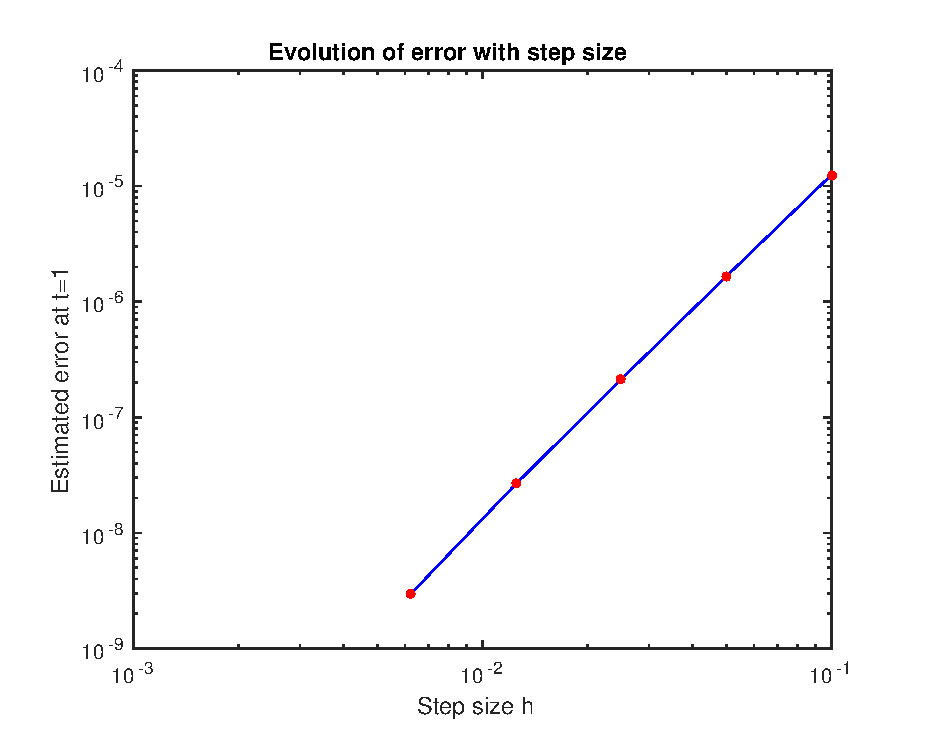
\includegraphics[width = 0.9\textwidth]{./a1.eps}
\caption{Loglog plot for empirical error of Runge-Kutta method on Van der Pol's equation}
\label{fig:a1}
\end{figure}

\FloatBarrier
We recognized the classical third order Runge-Kutta method and the order can be obtained analytically. This experiment confirms very well the results on a practical example. Here below is the Matlab code we used to estimate the order of the method.

\lstinputlisting{LAB2A.m}

